% @Author: YangZhou
% @Date:   2017-06-20 20:27:38
% @Last Modified by:   YangZhou
% @Last Modified time: 2017-08-12 14:18:46
\documentclass[%
 reprint,
 amsmath,amssymb,
 aps,
 prb,
]{revtex4-1}
\preprint{APS/123-QED}
\usepackage{graphicx}% Include figure files
\usepackage{bm}% bold math
\newcommand{\angstrom}{\mbox{\normalfont\AA}}
\newcommand{\bii}{$\beta-Bi_4 I_4$\;}
\begin{document}
\title{Ultra low thermal conductivity of quasi 1D bulk material \bii}
\author{Yang Zhou${}^{1,3}$}
\author{Zhi-Xin Guo${}^{2}$}
\author{Shi-you Chen${}^{1}$}
\author{Hongjun Xiang${}^{1}$}
\author{Xin-Gao Gong${}^{1,3}$}
\email{xggong@fudan.edu.cn}
\affiliation{%
  ${}^1$Key Laboratory for Computational Physical Science (Ministry of Education), State Key Laboratory of Surface Physics and Department of Physics, Fudan University, Shanghai 200433, China\\
  ${}^2$Department of Physics, Xiangtan University, Xiangtan 411105, China\\
  ${}^3$Collaborative Innovation Center of Advanced Microstructures, Nanjing 210093, Jiangsu, China
}%
\begin{abstract}
  The thermal transportation properties of recently synthesized quasi-1D bulk \bii  is explored from first principle. The thermal conductivity of this system is found rather low because of the phonon localization caused by the low-dimension nature and large anharmonic scattering of phonons. Detailed analysis of lattice dynamic calculation is applied to explain the origin of the anharmonic effects. The Seebeck coefficients and electric conductance are calculated from first principle and then ZT value is given. We found \bii  is actually potential for the application of thermoelectric. This research could be a guidance for further exploring of advanced low thermal conductivity materials.
  \begin{description}
    \item[Keywords]
          Thermal conductivity, quasi-1D,\bii, thermoelectric, phonons
  \end{description}
\end{abstract}

\maketitle

\section{INTRODUCTION}

Thermoelectric (TE) materials can directly convert heat into electricity or vice versa and, consequently, have attracted wide attention for applications in energy harvesting, and solid state cooling that does not require refrigerants \cite{Majumdar2004,Zebarjadi2012}. The figure of merit for thermoelectric performance is $ZT= S^2 \sigma T/(\kappa_L+\kappa_{el})$ , where S and $\sigma$ are the Seebeck coefficient and electrical conductivity, and $\kappa_L$ and $\kappa_{el}$ are the lattice and electronic thermal conductivities, respectively. Controlling of the power factor and the reduction of thermal conductivity due to phonon scattering are available ways to overcome the limits of the current ZT value. However, it is very difficult to significantly improve the thermoelectric performance of conventional materials because the $\sigma$, S and $\kappa_L$ are coupled unfavorably. For instance, a high electrical conductivity usually leads to a low Seebeck coefficient and a high electrical thermal conductivity, both of which are undesirable for thermoelectric applications.

It is well known that one of the promising methods for the achievement of highly efficient thermoelectric properties is to construct low-dimensional nanostructures which favors the surface scattering of phonons. Hicks et al. \cite{Hicks1993} theoretically predicated that low-dimensional structures may increase the ZT value by reducing lattice thermal conductivity with phonon-boundary scattering. Since then, a strong research activity has been focused on the low-dimensional structures, such as superlattices\cite{Balandin2003,Zhou2009}, nanowires(NWs)\cite{Zhang2009,Yan2008}, nanoribbons\cite{Xie2012,Sevincli2013,Jiang2010} , nanocomposites\cite{Joshi2011,Liu2011}, etc. for thermoelectric applications. For example, silicon nanowire has large ZT improvement than bulk systems because the quantum confinement reduce much of the thermal conductivity while has little influence with electronic properties\cite{Boukai2008,Hochbaum2008}. But nanowires are not easy to produced and are not practical in the application of thermoelectric application which needs a large bunch of nanowires to realize its function. Quasi-1D bulk materials that are made of weekly coupled 1D stripe block could solve this problem because they can be synthesized with chemical approaches while may be similar to that of nanowire bunch in the aspect of thermal conductivity.

\bii is a recently synthesized bulk material with quasi-1D structure\cite{Autes2015}. It is wealthy  investigating the thermal properties of \bii to see whether it has the nature of nanowire which may largely reduce the lattice thermal conductivity of the system. In this work, we have employed first-principles lattice-dynamics calculations of bulk \bii and found it��s indeed low thermal conductive and dynamical analysis and anharmonic analysis are applied to reveal the origin of the low thermal conductivity. Finally, the thermoelectric properties are predicted. This paper will be arranged as follows: in section I the computational method detail will be introduced and then in section II the results of phonon properties and thermal conductivity will be discussed. In section III the electrical properties will be explored. This work could give a new guidance for the low thermal conductivity materials searching.

\section{COMPUTATIONAL DETAILS}

Density functional theory(DFT) calculations are carried out by using the Vienna ab initio Simulation Package(VASP)\cite{Kresse1999}. The exchange and correlation interactions between electrons are described by the Perdew, Burke, and Ernzerhof functional(PBE)\cite{Perdew1996}. The projector augmented wave(PAW)\cite{Blochl1994} pseudopotential is adopted to model the interaction between electrons and ions. The energy cutoff is chosen to be 520 eV for the expansion of the wave function by plane-wave basis sets. The structure of bulk \bii is fully Relaxed with a k-point mesh of $4 \times 4 \times 4$.

Thermal conductivity the system is calculated by using Boltzmann Transportation Equation with relaxation time approximation as implemented in ShengBTE\cite{Li2014}, in which thermal conductivity tensor is given by

\begin{equation}
  K_{\alpha \beta}= \frac{1}{N_q V} \sum_{q\sigma} c_{q\sigma} v_{q\sigma,\alpha} v_{q \sigma,\beta} \tau_{q\sigma}
\end{equation}

The calculations of $c_{q\sigma}$ , $v_{q\sigma,\alpha}$, and $\tau_{q\sigma}$ require second- and third-order force constants (FCs) as inputs. Both second- and third-order FCs are extracted from density functional theory computations by using the finite displacement method. The FCs are calculated with $4 \times 2 \times 2$ supercell with a $3\times 3 \times 3$ Monkhorst-Pack k-point mesh. The phonon dispersion and states density are calculated with Phonopy\cite{Togo2008} with second order force constants. The interaction range of third-order FCs is truncated up to 4th neighbor.

\begin{figure}[b]
  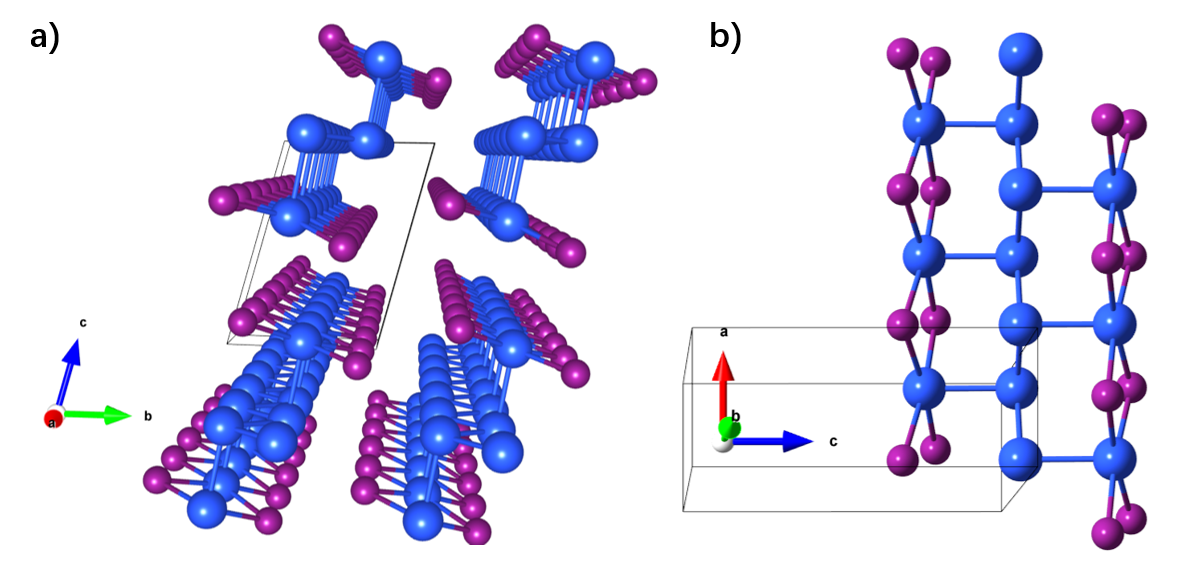
\includegraphics[width=0.48\textwidth]{images/structure}
  \caption{\label{fig:structure} (color online) Crystal structure of \bii. a) the perspective view of the bulk structure. Bi atoms are in blue and I atoms in purple. The crystal axes in the structure are chosen to match the stripe direction, in order to facilitate the calculation of thermal conductivity along the stripe. b) the side view of an individual chain-like stripe.}
\end{figure}


The thermoelectric properties including Seebeck coefficients and electric thermal conductivity are calculated with Boltzmann transportation equation(BTE) realized in Boltztrap\cite{Madsen2006} with eigenvectors extracted from VASP with k-point mesh of $14 \times 14 \times 14$.


\section{RESULTS AND DISCCUSION}

Bulk \bii is consist of weakly bounded 1D strips. As shown in Fig.~\ref{fig:structure}, the optimized configuration of the Bulk \bii possesses C2/m symmetry (space group no. 12) with a monoclinic lattice. The obtained lattice constants along the three lattice vectors are $4.445\angstrom$ ,$8.122\angstrom$,$11.057\angstrom$, and the volume of unit cell is $370.33 \angstrom^3$ which are in reasonable agreement with the experiment\cite{Autes2015}.

To confirm the dynamical stability of bulk \bii, phonon dispersion is calculated in the framework of the frozen phonon method\cite{Ihm1981}. The phonon dispersion along the high symmetrical path of the Brillouin zone and phonon states density are plotted in Fig.~\ref{fig:phonon}. No appreciable imaginary modes are found in the first Brillouin zone, suggesting that the bulk  \bii is dynamically stable.

\begin{figure}
  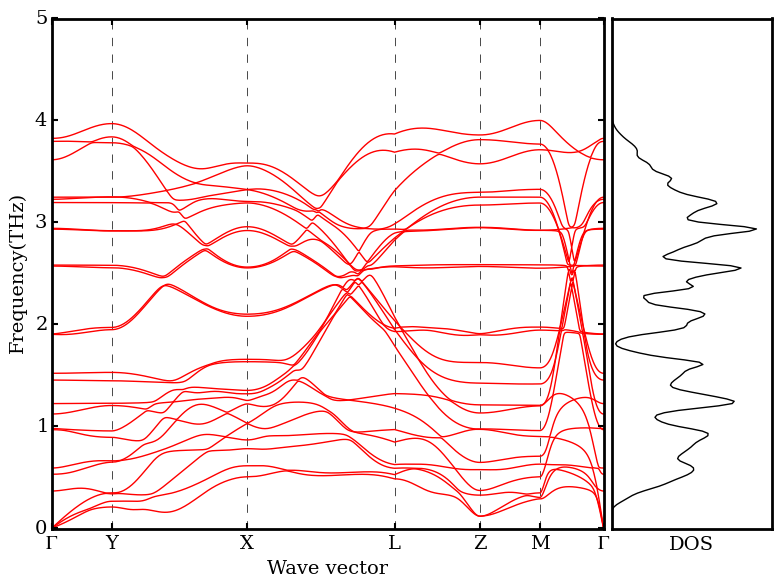
\includegraphics[width=0.48\textwidth]{images/phonon}
  \caption{\label{fig:phonon} (color online) Phonon dispersion along the high symmetric k-point path in the first Brillouin zone, along with phonon density of states.}
\end{figure}

To further study its thermal stability at finite-temperature, we performed ab initio molecular dynamics (MD) simulations at typical temperatures and the results of Mean Square Displacement(MSD)\cite{Michalet2010} are shown in FIG.\ref{fig:msd}. The MSD is defined as

\begin{equation}
  MSD= \langle |\mathbf{r}(t)-\mathbf{r}(0)|^2 \rangle
\end{equation}

where$\langle ... \rangle$ means the average of all the atoms.

\begin{figure}
  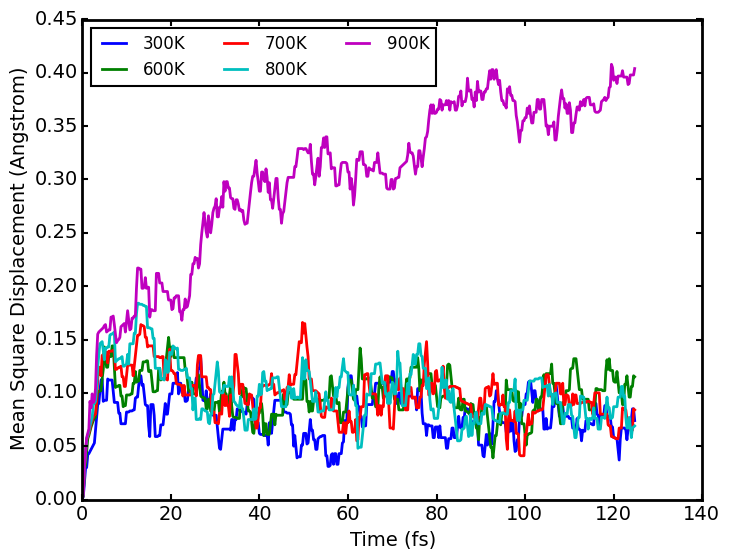
\includegraphics[width=0.48\textwidth]{images/msd}
  \caption{\label{fig:msd} (color online) Mean Square Displacement(MSD) vs. time under various temperature measured through ab-initial molecular dynamics. The continuous increasing of MSD at 900K means a phase transition between 800K and 900K.
  }
\end{figure}

For solids the MSD does not change while for liquids and gas it changes linearly with time. Therefore, the bulk \bii is thermally stable in a wide temperature range from 300 K to 800 K.

However, the structure starts melting when heated to 900 K. Thus we only concentrated on the trusted temperature range ($300K - 800K$), and choose 300 K as a typical temperature to perform the thermal conductivity calculations.



To obtain reliable results of thermal conductivity, the convergence dependence to q points density has to be tested. FIG.\ref{fig:convergence}a shows the convergence of thermal conductivity on $64 \times N \times N$ q points with N increase from 2 to 8. The TC shows its convergence at N=4, above witch the result changes a little but not the computational effort, so we choose the number of transverse q points to be both 4. Besides, the convergence on $N_x \times 4 \times 4$ q points with N increase from 16 to 1024 is also tested as in FIG.\ref{fig:convergence}b. The result of $N_x=200$ could be a good estimate of the converged result and we choose it to calculate TC only for the trends of TC on other properties like temperature et. al to save computer resources. FIG.\ref{fig:convergence}c shows the convergence on phonon cut off free path. The exact convergence could not be obtained even at $N_x=1024$ due to the abnormally large lifetime of long wave phonons show in FIG.\ref{fig:convergence}d, which always exist in low dimensional materials. However, a lot of research shows the relation of TC and phonon cut off free path obeys the rules of \cite{Schelling2002}

\begin{equation}
  \frac{1}{\kappa}=\frac{\alpha}{L}+\frac{1}{\kappa_\infty}
\end{equation}

and FIG.\ref{fig:convergence}e verifies that it also make sense in bulk \bii and the calculated results are over estimated. As the conclusion, the calculated results of thermal conductivity are not converged even in extremely dense q points, however they can be used as upper limited estimates of the exact results.

\begin{figure}[b]
  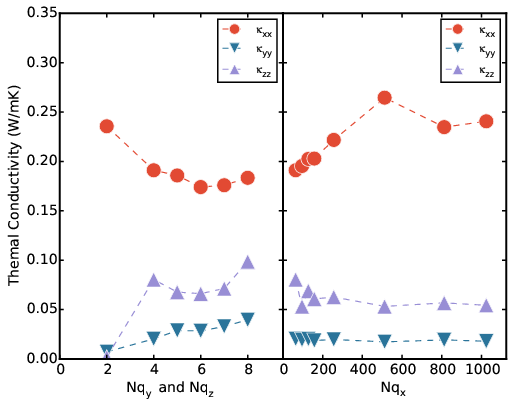
\includegraphics[width=0.48\textwidth]{images/convergence}
  \caption{\label{fig:convergence} (color online) Thermal conductivity(TC) convergence vs. q points of bulk \bii. a) Thermal conductivity convergence with $64 \times N \times N$ q points with N increase from 2 to 8. Although not obviously a convergence is reached, the result of N=4 is proved to be a reasonable approximation of convergent result. b) Thermal conductivity convergence with $N_x \times 4 \times 4$ q points with N increase from 16 to 1024. The convergence along the stripe direction is difficult to obtain because of the phonon life time divergence nature of 1D materials and the unreachable mean free path of them.
  }
\end{figure}

The thermal conductivity of \bii is extremely low and anisotropic as shown in FIG.\ref{fig:kappa}. The TC values decreases with increasing temperature and obeys the rule of $1/T$, and the largest value at 300K is much less than $1 W/mK$. The TC along the stripes are almost 3 times that of the transverse value which may result from the nature the quasi-1D structure.

Mode localization of phonons is believed to account for low thermal conductivity in this quasi-1D bulk system. To understand the underlying physical mechanism of localization of phonons on thermal conductivity, we have carried out a vibrational eigen-mode analysis. Mode localization can be quantitatively characterized by$P_{k\sigma}$, the participation ratio\cite{Huberman2013} for each eigen-mode $k\sigma$,

\begin{equation}
  P_{k\sigma}=\frac{1}{N \sum_s (\epsilon_{k\sigma}^* (s) \cdot \epsilon_{k\sigma} (s))^2}
\end{equation}

where N is the total number of atoms and $\epsilon_{k\sigma} (s)$ is the complex amplitude of atom s for eigen-mode $k\sigma$. The participation ratio presents the fraction of atoms participating in a given mode and effectively indicates the localized modes with $O(1/N)$ and delocalized modes with $O (1)$. It can provide a more detailed information about the localization effect to each mode. The eigenvectors and frequencies are obtained using Phonopy\cite{Togo2008} with $3\times2\times2$ supercell and $15\times15\times15$ mesh sampling. FIG.\ref{fig:phonon} shows the participation ratio of \bii. A lot of phonons have participation ratio below 0.5 which means they are strongly localized and lost the capability to carry energy and they have little contribution to thermal conductivity.

\begin{figure}[b]
  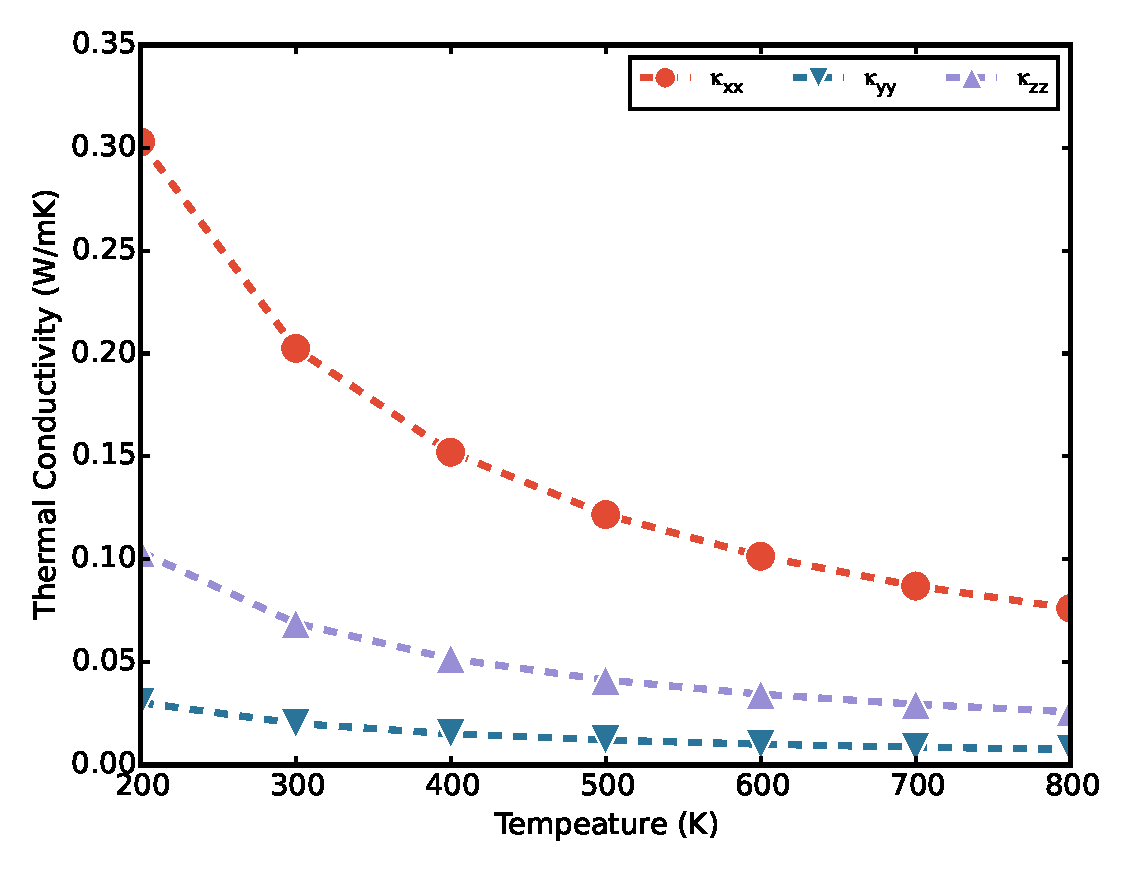
\includegraphics[width=0.48\textwidth]{images/kappa_t}
  \caption{\label{fig:kappa} (color online)Thermal conductivity vs. temperature along the three lattice vectors. The TCs are found to be pretty low. The highly anisotropic structure result in the understandable anisotropic but unexpectedly, the TCs along the stripe and along the inter-stripe direction y are pretty close while the TC along the other inter-stripe direction z is much higher.
  }
\end{figure}

Large anharmonic would be another key factor that account for the low thermal conductivity. FIG.\ref{fig:gv} shows the group velocity of the phonons. Although the frequencies are pretty low (phonons are pretty soft), the group velocities are not so small witch can be understood by the steep phonon dispersion, for example, along the path $\Gamma M$. The maximum group velocity is comparable to that of graphene witch possesses the largest thermal conductivity so far. So group velocity is not responsible for the low TC. The large Gruneisen parameters\cite{Hasegawa1980} showed in FIG.\ref{fig:phonon}b means pretty large anharmonic effects in \bii which suggest strongly three-phonon scattering effects\cite{Hungary1985Phonon}. FIG.\ref{fig:phonon}a shows the three-phonon scattering relaxation time of all the phonons. The mean free path are also show in FIG.7b.Except for the long wave ones, all the life time are pretty small and this is exactly the origin of the low TC. The scattering strength show in FIG.\ref{fig:phonon}a also shows large scattering of phonons.

\begin{figure}[b]
  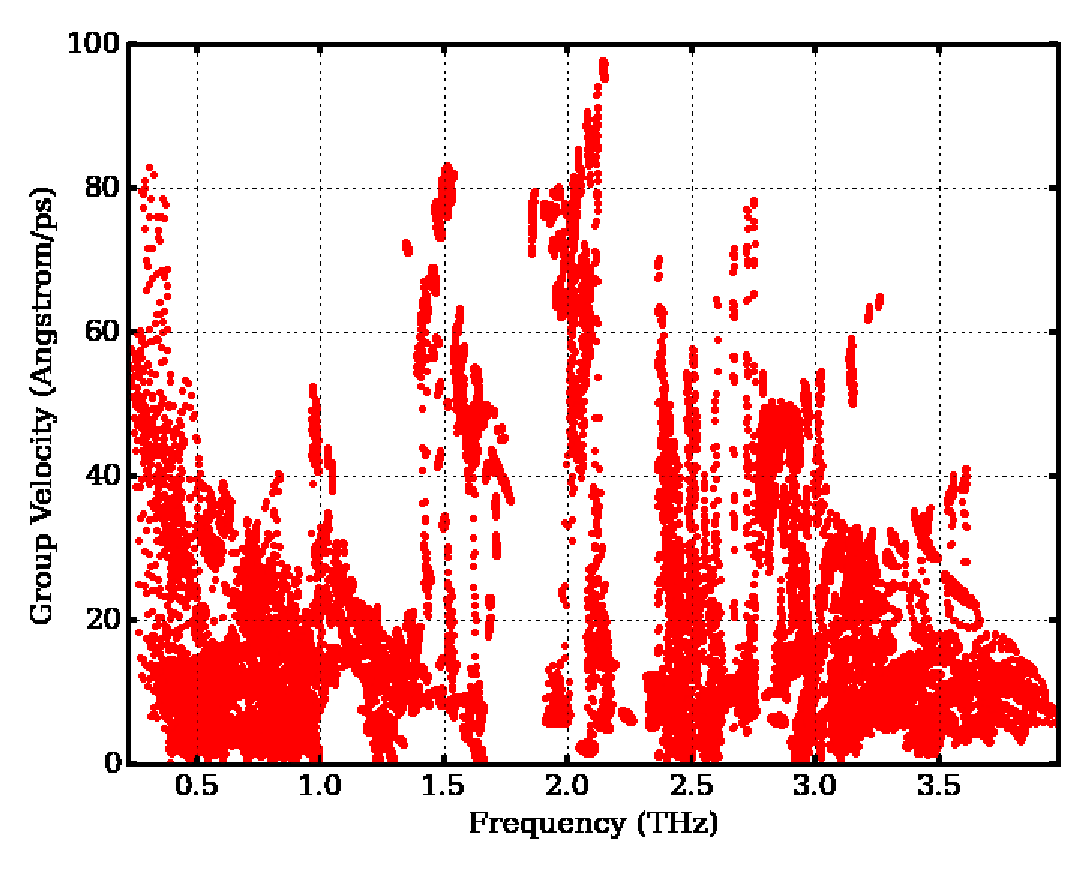
\includegraphics[width=0.48\textwidth]{images/gv}
  \caption{\label{fig:gv} (color online) Phonon group velocity of bulk \bii. Although the frequencies are pretty low (phonons are pretty soft), the group velocities are not so small witch can be understood by the steep phonon dispersion, for example, along the path $\Gamma M$. The maximum group velocity is comparable to that of graphene witch possesses the largest thermal conductivity so far.
  }
\end{figure}

Low TC means the potential of applications in thermoelectric field and \bii is predicted to be a good thermoelectric material. FIG.\ref{fig:phonon}a shows Seebeck coefficient S at different temperatures. The typical values are in the range of several mV/K and are comparable with that of SnSe. Seebeck coefficient are sensitive to temperature while FIG.\ref{fig:phonon}b shows that electric conduction $\sigma$ are not. The power factor $S^2 \sigma$ are shown in FIG.\ref{fig:phonon}c. Although Seebeck coefficient is smaller at 700K, power factor is higher because of the rise and fall of $\sigma$ around fermi level. However $\kappa{_el}$ is also higher at 700K which eliminate the difference. The electric thermal conductivity is comparable at all the temperature and is even higher, which dominant at high temperature as shown in FIG.\ref{fig:phonon}a. At this point all the factors of figure ZT of merit are collected and the final results are shown in FIG.\ref{fig:phonon}b. After some n-doping or p-doping, ZT reaches its maximum and the best values could be obtained at high temperature. At 700K this ZT value is around 0.8 and this is not bad for the application of thermoelectric energy translation.

\section{CONCLUSIONS}

To summarize, in this work, we propose to study the thermal transportation properties of quasi-1D bulk material \bii from first principle. Our numerical results demonstrate that \bii possess thermal conductivity as low as $0.5 W/mK$ and its TC are strongly anisotropic and the direction along the 1D blocks is the most thermal conductive. The low thermal conductivity origins from the phonon mode localization caused by the week interaction between the 1D blocks and also origins from large anharmonic effect which accounts for the large three-phonon scatter rate. The potential of \bii in thermoelectric application is also inspected and we found although the Seebeck coefficient is large, the low electric conductance limits the figure of merit ZT to be around 0.8 which is comparable to the current thermoelectric material $Bi_2 Te_3$\cite{Osterhage2014} but not stand for the best catalog in this field. Our research shows that quasi-1D bulk materials have low thermal conductivity with large probability and is a guidance for searching of new thermoelectric materials in the future.

\quad \\
\section{ACKNOWLEGEMENTS}
This paper was partially supported by the National Natural Science Foundation of China, the Special Funds for Major State Basic Research, the Foundation for the Author of National Excellent Doctoral Dissertation of China, the Program for Professor of Special Appointment at Shanghai Institutions of Higher Learning, and the Research Program of Shanghai Municipality and the Ministry of Education.


\bibliography{ref}
\end{document}